\begin{center}
{\textbf{Vendredi 20 août : Entraînement et après-midi détente}}
\end{center}
\vspace{2mm}

Ça y est, l’heure est venue pour les élèves de mettre en œuvre ce qu’ils ont appris jusqu’ici. Comme durant une vraie olympiade, les stagiaires passent la matinée à réfléchir sur une série de 4 problèmes complexes, qui leur permettent de faire usage des techniques et idées qui leur ont été transmises durant les cours. Les élèves travaillent de 9 h à 12 h (sauf le groupe D, qui doit se lever une heure plus tôt.) D’habitude animées, les salles de classe sont calmes aujourd’hui, les élèves — sérieux et concentrés. Heureusement, l’atmosphère studieuse est un peu adoucie par les mélodies du musical „Cats”, que des jeunes choristes répètent dans les étages supérieurs. Manifestement, les chants sont aussi accompagnés de danses énergiques.

Après cette séance entraînement, les élèves ont enfin un après-midi complet de détente.

Au programme : Sporz avec Aurélien (un jeu ressemblant vaguement au loup-garou mais avec des astronautes dans un vaisseau spatial infecté), jeux de société avec Jérémy, ou encore un Stratego géant organisé par Tris’Tanos, Alexand’Hercules et Pi’Hermès ! Pendant que les premiers courent après les mutants et que les seconds font Bang sur Bang, trois tribus se combattent avec acharnement pour pouvoir défier les dieux à de petits jeux et obtenir des indices pour trouver l’assassin de Victor. Précisons que si l’assassin n’avait pas aussi volé le goûter, il n’est pas certain que les élèves aient été aussi motivés…

\begin{figure}[H]
\centering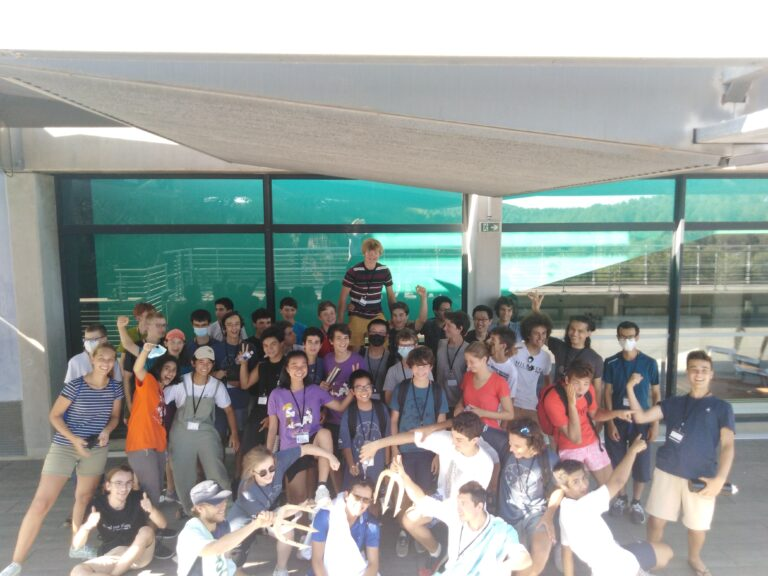
\includegraphics[width=6cm]{CR-20-0.jpg}
\caption{Les participants au Stratego se réjouissent pour le goûter (juste avant d’apprendre que celui-ci a une demi-heure de retard…)}
\end{figure}

Pendant ce temps, les animatheurs corrigent multiples copies qui leur ont été rendues. Celles-ci doivent être prêtes avant 20 h, l’heure prévue de la correction.